\chapter{Descrizione dello stage}
\label{cap:descrizione-stage}

In questo capitolo, viene fornita una spiegazione più dettagliata del progetto e della relativa organizzazione.

\section{Introduzione al progetto}

Uno dei principali mercati dove opera Euronovate è il mercato dei device di firma grafometrica
dotati di un monitor da 10 pollici multi-touch.\\ Questi dispositivi USB possono essere utilizzati
per molteplici scopi oltre all'inserimento di una firma in un documento, nel tempo l'azienda ha visto
realizzare sistemi di presentazioni slideshow, digital signage, questionari di valutazione e form
per l'aggiornamento delle anagrafiche.\\ Oggi Euronovate vuole spingersi ulteriormente nel mondo dei
multimedia e utilizzare il device di firma ENSign 11 per l'intrattenimento videoludico.\\
L'obiettivo dello stage è apprendere le nozioni dello sviluppo di applicazioni desktop e di integrazioni di dispositivi fisici, lavorando in team e seguendo una pianificazione
settimanale delle attività.\\ 
Ulteriori feature di prodotto possono essere proposte dallo stagista e saranno valutate dal tutor.

\section{Analisi preventiva dei rischi}

Durante la fase di analisi iniziale sono stati individuati alcuni possibili rischi a cui si potrà andare incontro.
Si è quindi proceduto a elaborare delle possibili soluzioni per far fronte a tali rischi.\\

\begin{risk}{Performance del simulatore hardware}
    \riskdescription{le performance del simulatore hardware e la comunicazione con questo potrebbero risultare lenti o non abbastanza buoni da causare il fallimento dei test}
    \risksolution{coinvolgimento del responsabile a capo del progetto relativo il simulatore hardware}
    \label{risk:hardware-simulator} 
\end{risk}

\section{Requisiti e obiettivi}


\section{Pianificazione}

\subsection{Fasi e dettagli}

In accordo con il tutor aziendale, si è deciso di suddividere il tirocinio nelle seguenti fasi:
\begin{itemize}
    \item Conoscenze generali, dal 2 Maggio al 5 Maggio.
    \item Formazione personale, dal 8 Maggio al 19 Maggio.
    \item Analisi dei Requisiti, dal 22 Maggio al 25 Maggio.
    \item Progettazione Tecnica, dal 25 Maggio al 2 Giugno.
    \item Codifica, dal 5 Giugno al 6 Luglio.
    \item Documentazione, dal 7 Luglio al 10 Luglio.
    \item Demo, l'11 Luglio.
\end{itemize}

\subsubsection{Conoscenze generali}
Questa fase, della durata di 4 giorni, ha previsto l'installazione degli ambienti di sviluppo e di versionamento, nonchè un approfondimento degli stessi. Inoltre, sono stati abilitati gli strumenti aziendali (account git, AWS, Verdaggio e GSuite) necessari per il tirocinio.
\subsubsection{Formazione personale}
In questa fase, durata 10 giorni, l'obiettivo era l'approfondimento dello sviluppo attraverso le tecnologie necessarie per il progetto.\\
In particolare, l'approfondimento riguardava ElectronJS per lo sviluppo dell'applicazione desktop, comprese le tecniche di comunicazione tra processi per il passaggio dei dati tra C++ e TypeScript. Inoltre, era necessario approfondire il funzionamento del framework Angular per la parte front-end dell'applicativo.\\
L'approfondimento di questa fase ha portato ad una piccola applicazione che comprendeva tutte le parti appena citate.
\subsubsection{Analisi dei Requisiti}
\subsubsection{Progettazione tecnica}
\subsubsection{Codifica}
\subsubsection{Documentazione}
\subsubsection{Demo}

\subsection{Supervisione e controllo}

\subsection{Diagramma di Gantt}
\begin{figure}[!h] 
    \centering 
    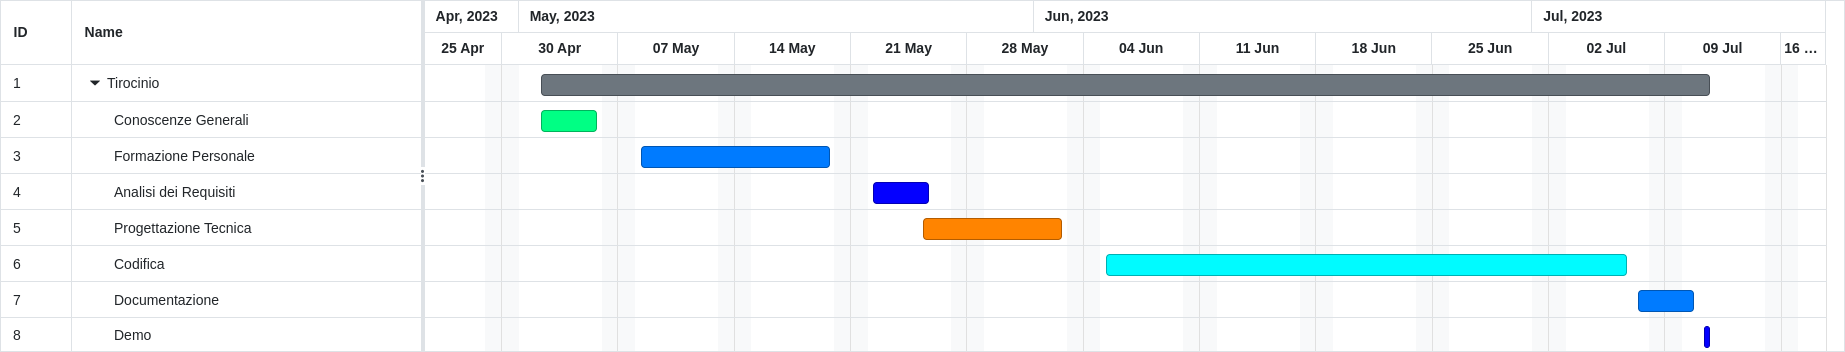
\includegraphics[width=350pt]{images/diagrammaGantt.png} 
    \caption{Diagramma di Gantt del tirocinio}
\end{figure}
